\documentclass[tikz, margin=3.14mm]{standalone}

\usepackage{tikz}
\usepackage{amsmath}
\usepackage{nicefrac}
\usetikzlibrary{backgrounds}

\begin{document}

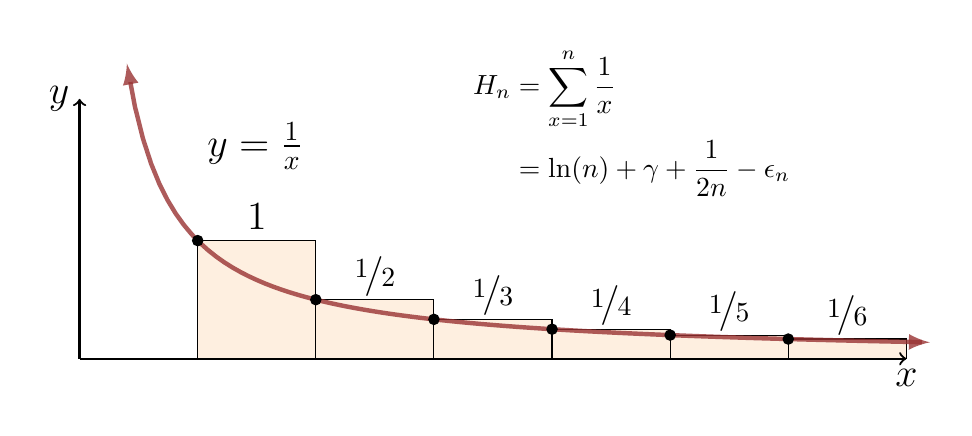
\begin{tikzpicture}[scale=1.5, font=\Large, background rectangle/.style={fill=white}, show background rectangle]

    % Draw the rectangles
    \foreach \x in {1, 2, 3, 4, 5, 6} {
        \draw[fill=yellow!40!red!10] (\x, 0) rectangle (\x+1, {1/\x});
    }

    % Define the function
    \draw[
        latex-latex, 
        domain=0.4:7.2, samples=100, ultra thick, red!50!black!80, opacity=.8] plot (\x, {1/\x});
    
    % Define the axis
    \draw[thick,->] (0,0) -- (7,0) node[anchor=north] {$x$};
    \draw[thick,->] (0,0) -- (0,2.2) node[anchor=east] {$y$};
    
    
    % Draw the points on the curve
    % \def\nodelabels{{"$1$", "$1/2$", "$1/3$", "$1/4$", "$1/5$", "$1/6$"}}
    \def\nodelabels{{"$1$", "$\nicefrac{1}{2}$", "$\nicefrac{1}{3}$", "$\nicefrac{1}{4}$", "$\nicefrac{1}{5}$", "$\nicefrac{1}{6}$"}}

    \foreach \x in {1, 2, 3, 4, 5, 6} {
        \filldraw (\x, {1/\x}) circle (1.25pt);
        % \node at (\x+0.5, 1/\x + .25) {\pgfmathparse\nodelabels[\x-1]\pgfmathresult};
        \node at (\x+0.5, {1/\x + 0.2}) {\pgfmathparse{\nodelabels[\x-1]}\pgfmathresult};
    }
    
    % Draw vertical lines from points to the x-axis
    \foreach \x in {1, 2, 3, 4, 5, 6} {
        \draw[dashed] (\x, {1/\x}) -- (\x, 0);
    }
    
    % Label for the curve
    \node at (1, 1.8) [anchor=west] {$y = \frac{1}{x}$};

    \node at (3.25, 2) [anchor=west] {
        ${\normalsize 
        \begin{aligned}
            H_n & = \sum_{x=1}^n \frac{1}{x} \\
            & = \ln(n) + \gamma + \frac{1}{2n} - \epsilon_n
        \end{aligned}}$};

    
\end{tikzpicture}

\end{document}
